\documentclass{article}

\usepackage{cite, enumitem, graphicx, hyperref, lipsum, subcaption, verbatim, wrapfig, rotating}
\usepackage[normalem]{ulem}
\usepackage[most]{tcolorbox}
\useunder{\uline}{\ul}{}

% code blocks
\definecolor{codecolor}{rgb}{0.95,0.95,0.92}
\newcommand{\textcode}[1]{\colorbox{color}{\texttt{#1}}}

\title{Plaint-or-Tweet}
\author{Tommaso Battistini, Edoardo De Matteis, Leonardo Emili, \\
Mirko Giacchini, Alessio Luciani}

\begin{document}
    \maketitle
    
    \section*{Introduction}
    For our final project we decided to implement some sentiment analysis techniques on social media data, and in particular on tweets from the social network Twitter. We used a dataset from Kaggle ~\cite{data:sentiment140} which contains 1.6 million tweets labelled as positive or negative (the dataset is balanced: there are 800k positive tweets and 800k negative tweets). We chose this topic because it is of course interesting from a research point of view, but it has also many applications in industry: for example we discovered some companies that provide sentiment analisys on social media as one of their main services ~\cite{startups:spiketrap} , these services are especially useful to other companies, for example to understand what their customers think about the release of new products (and in many similar scenarios). 

    \section*{Models}
    As we have seen during coursework, the na\"ive Bayes classifier has proved to be a good model for spam classification, and it is therefore reasonable to expect good results also in sentiment analysis. We decided to implement many variations of na\"ive Bayes to have a deeper understanding on how the representation of a tweet (and in general of a text) affects the performances of this class of models.
    \subsection*{Classic na\"ive Bayes}
    We implemented the multivariate bernoulli event model, in which each tweet $T$ is associated to a boolean vector $V$ and $V[i]=1$ if and only if the $i$-th word of the dictionary is present in tweet $T$.
    
    Another classical model we implemented is the multinomial event model: for each tweet we create a vector where the $i$-th value is the number of times the $i$-th word of the dictionary appears inside the tweet; note that this representation is a bit different from the one seen during coursework but we get equivalent formulas for the parameters and this representation makes the implementation of the model easier. In the multinomial event model we also tried to associate to each word its tf-idf score instead of the number of occurrences: the tf-idf value is a score associated to a word inside a tweet, that increases the more the word is repeated inside the tweet and decreases the more the word is repeated in the whole training set. This is an improper way of using the multinomial event model because we are not using vectors of positive integers, but we are using positive real values; however this variation has been used a lot in practice and it seems to perform well.
    
    In both these models, we also tried to use the n-grams: we don't consider only the single words as features, but also groups of adjacent words (for example with bigrams, we consider couple of adjacent words as features).
    
    \subsection*{Embeddings}
    A relatively new idea that has been really successful in natural language processing, is the one of word embeddings: we associate to each word a vector of real values, learned via deep learning techniques. The two most common algorithms to create word embeddings are FastText and Word2Vec, we tried both of them to get the embeddings of words\footnote{Since their performance is basically the same, in the tests we show just FastText results}, to get the embedding of a tweet we average the embeddings of the words it contains. To make predictions from the tweet embeddings we used three versions of na\"ive Bayes. We tried the multinomial event model on the raw values of the embedding, the only difficulty here is that the embedding might contain negative values and this could result in negative probabilities in the multinomial event model: to fix this, we translate all the values to make them positive (we do this looking at the minimum value in the training set, for each feature), the intuition behind this model is to consider the values of the embeddings as score (as it is done with tf-idf), but of course this might not be true in general, since the main property of word embeddings is that similar words will be close to each other. We also tried the multinomial event model discretizing each features in $k$ buckets (and in this case, the features will not ``mix up'', i.e. each feature will be treated indipendently), this is something often done in the multinomial event model when dealing with continuous values, so we expected some decent results from this model. The last model we used is a gaussian na\"ive Bayes: assuming that the features are gaussian is another common way to deal with continuous values in na\"ive Bayes, however in this case the values are artificial and we didn't expect them to be gaussian hence from this model we expected bad results.
    
    Word embeddings are generally used as input for complex models such as neural networks, we thought it was interesting to see if also simpler models such as na\"ive Bayes can take profit from these successful representations.
    
    Note that there are many other ways to create the embedding of a tweet from the word embeddings, for example we could do a weighted average (weighting the words according to some score, for example tf-idf), or we could concatenate the word embeddings (truncating too long tweets, and padding too short tweets).
    
    \subsection*{Notes on implementation}
    The core of the models has been implemented from scratch, but for the data preparation we used some scikit-learn function: for example we implemented the multinomial event model assuming in input vectors of positive values, and we used a scikit-learn function to transform a tweet to a vector (of frequencies or tf-idf scores). Since the dataset is really large, the efficiency of the learning and testing procedures has been a critical factor to take into account. We managed to get reasonably efficient algorithms leveraging numpy and scipy functions: speaking at a very high level, the key idea has been to compute most of the needed values across all the training set (or all the test set) instead of iterating over the train sample (or test sample) and compute such values in a trivial way.

    \section*{Preprocessing}

    Data preprocessing is a vital step in any Machine Learning pipeline, and it is particularly meaningful when dealing with natural language.
    The fact is that natural language is inherently ambiguous, and in many NLP tasks, we care a lot about the quality of our data which has to be high enough in order to achieve good results.
    In this case, we tackled the Sentiment Analysis task on the Twitter dataset which consists of a collection of user tweets with their annotated sentiment (either positive or negative) and some additional information such as the tweet identifier, the author, etc \dots
    
    As the first step, we cleaned the dataset from all the columns and retained only those related to text and (ground truth) sentiment annotation. We even performed some minor transformations on class labels which were originally defined in \{0,4\} to have values in \{0,1\}.
    
    \begin{figure}[h!t]
        \centering
        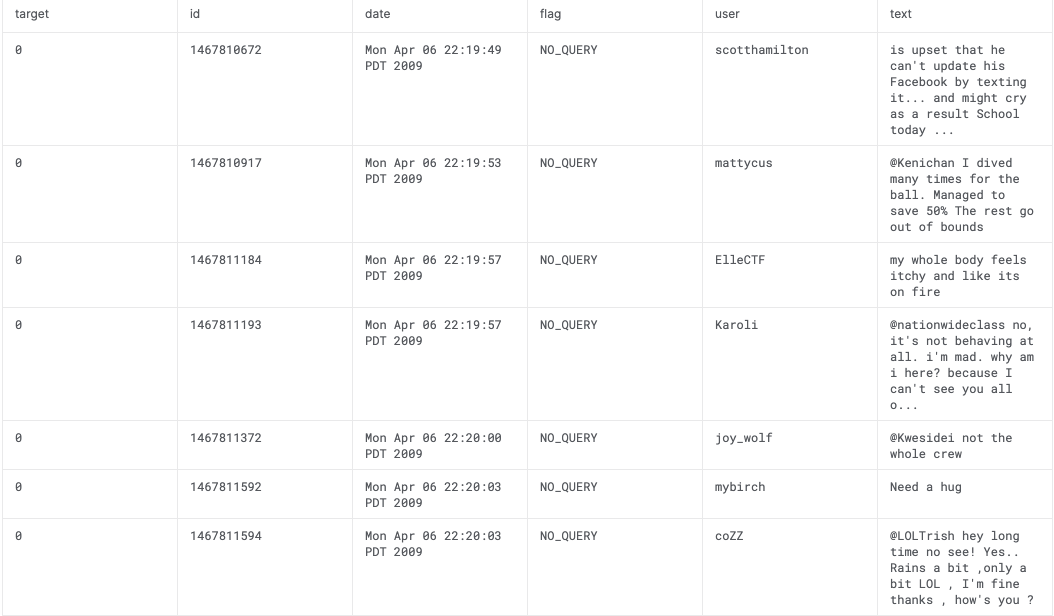
\includegraphics[scale=0.32]{twitter_overview.png}
        \caption{Overview of the Twitter dataset.}
        \label{fig:TWITTER_OVERVIEW}
    \end{figure}
    
    We noticed that users tend to make mistakes when posting new tweets either because of typos or replacement of english words with abbreviations or idiomatical terms (e.g. slang or internet jargon).
    Therefore, we chose to perform major treatments on our data and tried to correct these errors in order to enhance the quality of our corpus (e.g. replace duplicated characters, 'hellooo' becomes 'helloo' and 'tooo much' becomes 'too much').
    
    We decided to apply lemmatization and tokenization, which are common operations in NLP tasks, on our dataset, and in order to do that we relied on the spaCy pipeline ~\cite{startups:spaCy} because of its efficiency and nowadays many companies that deal with natural language processing have chosen to use it~\cite{data:companies_using_spacy}.
    
    While it is common to tokenize sentences into words before passing them to a model, we thought it would be interesting to use lemmas instead of the original words since different variations of the original lemma have the same meaning (e.g. 'be', 'been' and 'am' refer to the same concept) and models should benefit from this process since they will have the chance to see multiple times the same lemma in different contexts.
    
    Moreover, we managed to filter out from our corpus those common words that do not contribute to adding meaning to our sentences: the so called stopwords.
    There is a plethora of valid collections of stop-words available on the web (e.g. NLTK~\cite{startups:nltk}, Gensim~\cite{startups:gensim}) and we decided to use those offered by spaCy.
    
    \subsection*{Effects of preprocessing}
    
    At first, we expected this process to lead to good results since it simplifies the problem by removing a possibly long list of words whose presence can be neglected, but we had to change our mind about that.
    
    Here in figure \ref{fig:PREPROCESSING_ROC} we can see some interesting results when testing our intuition on data preprocessing either for the multivariate Bernoulli or the multinomial na\"ive Bayes with word embeddings. 
    Nevertheless, if we observe these ROC curves we discover some unexpected results: both the models achieved the best results when trained on non-preprocessed data.
    %\clearpage
    
    
    \begin{figure}[h!t]
        \centering
        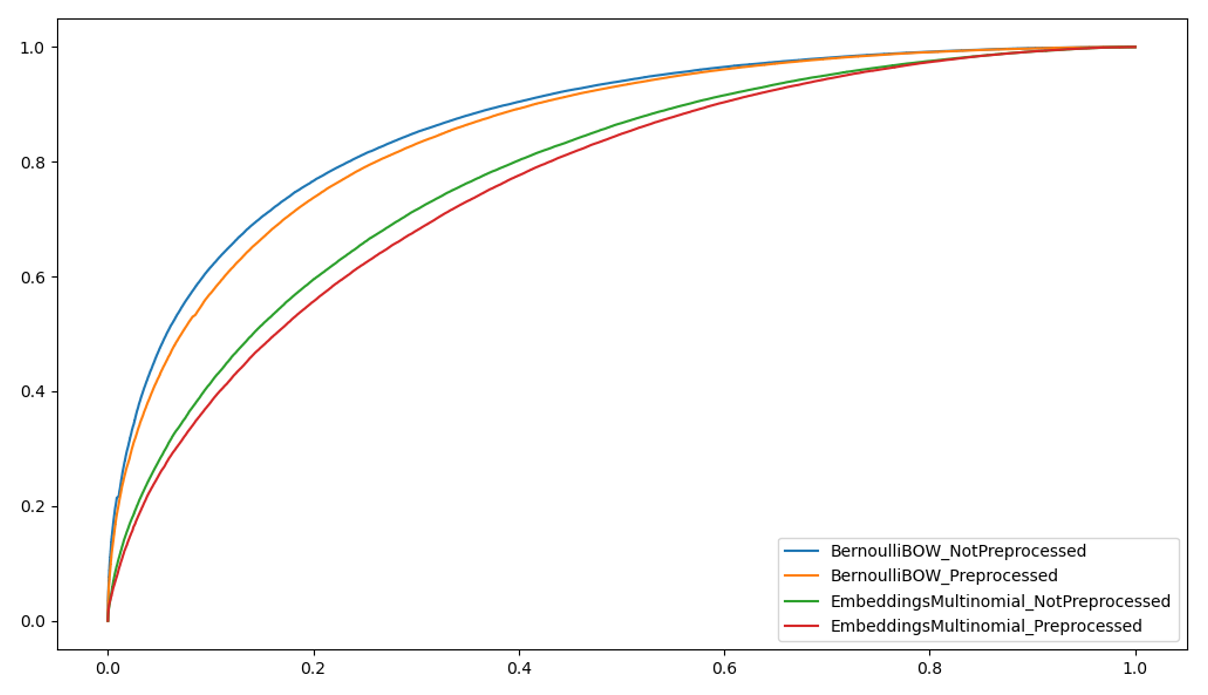
\includegraphics[width=11cm]{../experiments/plots/preprocessing.png}
        \caption{ROC curve with 80\% training and 20\% test.}
        \label{fig:PREPROCESSING_ROC}
    \end{figure}
    
    
    We struggled to understand why and we found two principal causes.
    First, lemmatization is not always a good idea and in some cases using the original words instead of their lemma is the best choice.
    More generally, this is a strong text manipulation technique and common sense tells us that if it does not allow us to gain a significant performance gain we should avoid it ~\cite{data:lemmatization_tips}. 
    Second, it is not always a good idea to remove stopwords especially if the stopwords come from a general dictionary, in fact some words considered stopwords in a context might be useful words in another context. 
    Using the spaCy stopwords the performance of our model decreased, instead using an ad-hoc set of stopwords (which contained only a few words such as articles and pronouns) we got some slightly better results compared to the case where no preprocessing at all is done (table \ref{tab:stopwords}).
    
    \begin{table}[h!t]
        \centering
        \caption{Comparing the results of preprocessing on our Bernoulli model. We randomly splitted the dataset in 80\% training set, 20\% test set.}
        \label{tab:stopwords}
        \begin{tabular}{c|c}
            \hline
            Preprocessing & Accuracy \\
            \hline 
            complete (spaCy pipeline) & 0.7690 \\ 
            none & 0.7828 \\ 
            ad-hoc stopwords removal & 0.7834 \\ 
            \hline
        \end{tabular}
    \end{table}
    
    
    \section*{Tests and metrics}

    \subsection*{Classic Na\"ive Bayes vs Embeddings}
    
    In figure \ref{fig:classic_nb_vs_embeddings} are shown the ROC curves obtained with the models without preprocessing, the dataset split is set to 80\% for the train set and 20\% for the test one.
    We can see how simpler approaches eventually bring the best results, in fact using word embeddings the final accuracy was much lower than the one obtained with the classic na\"ive Bayes with bag of words. From these tests it looks like na\"ive Bayes can't exploit the properties of word embeddings at their best. It is also interesting to note how using the Gaussian model with embeddings turned out to be the worst model, as the values in the embeddings are probably not gaussian.
    
    \begin{figure}[h!t]
        \centering
        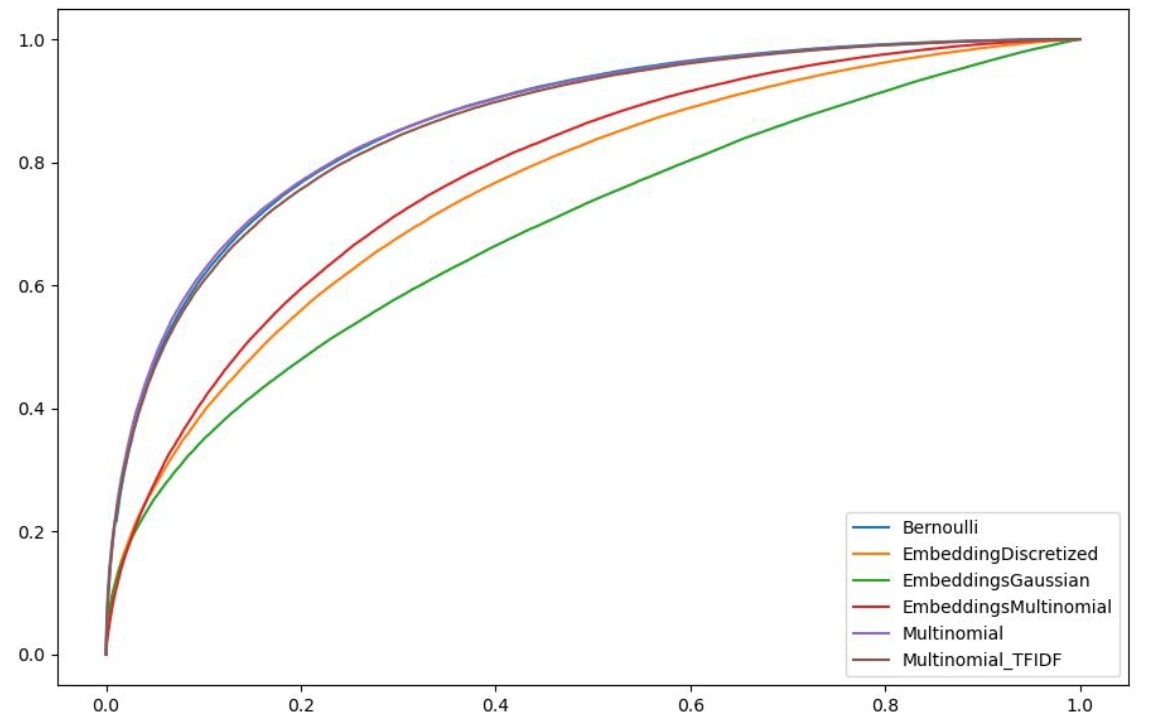
\includegraphics[scale=0.50]{../experiments/plots/classic_nb_vs_embeddings}
        \caption{ROC curves that compare the classic Na\"ive Bayes models and
        word embedding approaches.}
        \label{fig:classic_nb_vs_embeddings}        
    \end{figure}
    
    Classical na\"ive Bayes are the best performing models so, focusing on them, some hyperparameter tuning has been applied. The intention has been to find the best n-grams to maximize the final results. In order to do that, 20\% of the dataset has been dedicated to the cross validation set (60\% to training, 20\% to test).
    In table \ref{tab:classic_nb_vs_embeddings} we can see some metrics. 
    All of their performances are very similar with around 80\% of Accuracy and F1-score and 88\% of AUROC. The best n-grams turned out to be (1-3)-grams (for Bernoulli and Multinomial with tf-idf) and (1-2)-grams for standard multinomial event model.
    
    \begin{table}[h!t]
        \centering
        \caption{Results obtained with bag of words Bernoulli and Multinomial models.}
        \label{tab:classic_nb_vs_embeddings}
        \begin{tabular}{c|ccc}
            \hline
            Model & Accuracy & F1 & AUROC \\
            \hline 
            Bernoulli & 0.797 & 0.799 & 0.880 \\ 
            Multinomial & 0.802 & 0.802 & 0.884 \\ 
            Multinomial TF-IDF & 0.805 & 0.804 & 0.886 \\ 
            \hline
        \end{tabular}
    \end{table}
    
    \subsection*{Kaggle notebooks}
    
    In this section we describe how we compared our models to a couple of top-rated notebooks on Kaggle.
    We also tried to run these notebooks without removing stopwords from their datasets hoping to gain some further insight on their role in the learning process. 
    
    The model we chose to compare to these notebooks is our best performing one: multinomial na\"ive Bayes with tf-idf. 
    The first selected notebook is the best one that uses this same technique ~\cite{startups:notebook1}, we resized our dataset split to match their and have a comparison as equal as possible.
    We were happy to see that their AUROC score was slightly lower than ours, as showed in \ref{tab:versus_metrics_NB}.
    However their performance fairly improved when no processing was applied.
    
    \begin{table}[h!t]
        \centering
        \caption{Model comparision with and without preprocessing.}
        \label{tab:versus_metrics_NB}
        \begin{tabular}{c|c}
            \hline
            Model & AUROC \\
            \hline 
            Notebook & 0.839 \\ 
            Us & 0.841 \\ 
            Notebook no preprocessing & 0.849 \\ 
            \hline
        \end{tabular}
    \end{table}
    
    We also wanted to see if more complex models could capture the irregularities in word embeddings better than ours na\"ive Bayes. 
    We looked for Kaggle notebooks with best results on word embeddings and found ~\cite{startups:notebook2} who is based on a LSTM neural network.
    We were truly surprised to see that its accuracy was lower than the one reached by our tf-idf model, scores are showed ay table \ref{tab:versus_metrics_FT}. 
    Anyway when emptying the lists of stopwords to be removed from the dataset and running the notebook again its accuracy enjoys a significant boost. 
    These results make us support the intuition that some stopwords contain useful information that we want to keep in our dataset. 
    
    \begin{table}[h!t]
        \centering
        \caption{Model comparision with and without stopword removal.}
        \label{tab:versus_metrics_FT}
        \begin{tabular}{c|c}
            \hline
            Model & Accuracy\\
            \hline 
            Notebook & 0.779 \\ 
            Us & 0.799 \\ 
            Notebook with stop-word & 0.816 \\ 
            \hline
        \end{tabular}
    \end{table}
    
    \subsection*{Further tests}
    We performed some unusual tests: we trained our model with a dataset and tested it against a different one. The motivation behind this test is the following: suppose we have a model which is good in sentiment analysis on tweets, and we would like to do sentiment analisys also on another social network but for which we don't have any data to train on (if we had even a small amount of data, we could try some transfer learning technique), then it is interesting to see if our model trained on twitter can give decent results also on the other social network, or if the results will be basically random.\\
    We used an IMDb dataset of cinematographic reviews ~\cite{data:imdb} and a Reddit one about various NFL games\footnote{In this dataset the label is a real value in [-1,1], we considered only the comments with absolute value greater than 0.5, and set their label either to 0 or 1} ~\cite{data:reddit}, results for the Multivariate Bernoulli event model Na\"ive Bayes (using (1,3)-gram\footnote{In a (1-3)-gram we consider 1,2 and 3-grams}) without preprocessing can be seen in figures \ref{fig:TwitterImdb} and \ref{fig:TwitterReddit}.
    
    \begin{figure}[h!t]
        \centering
        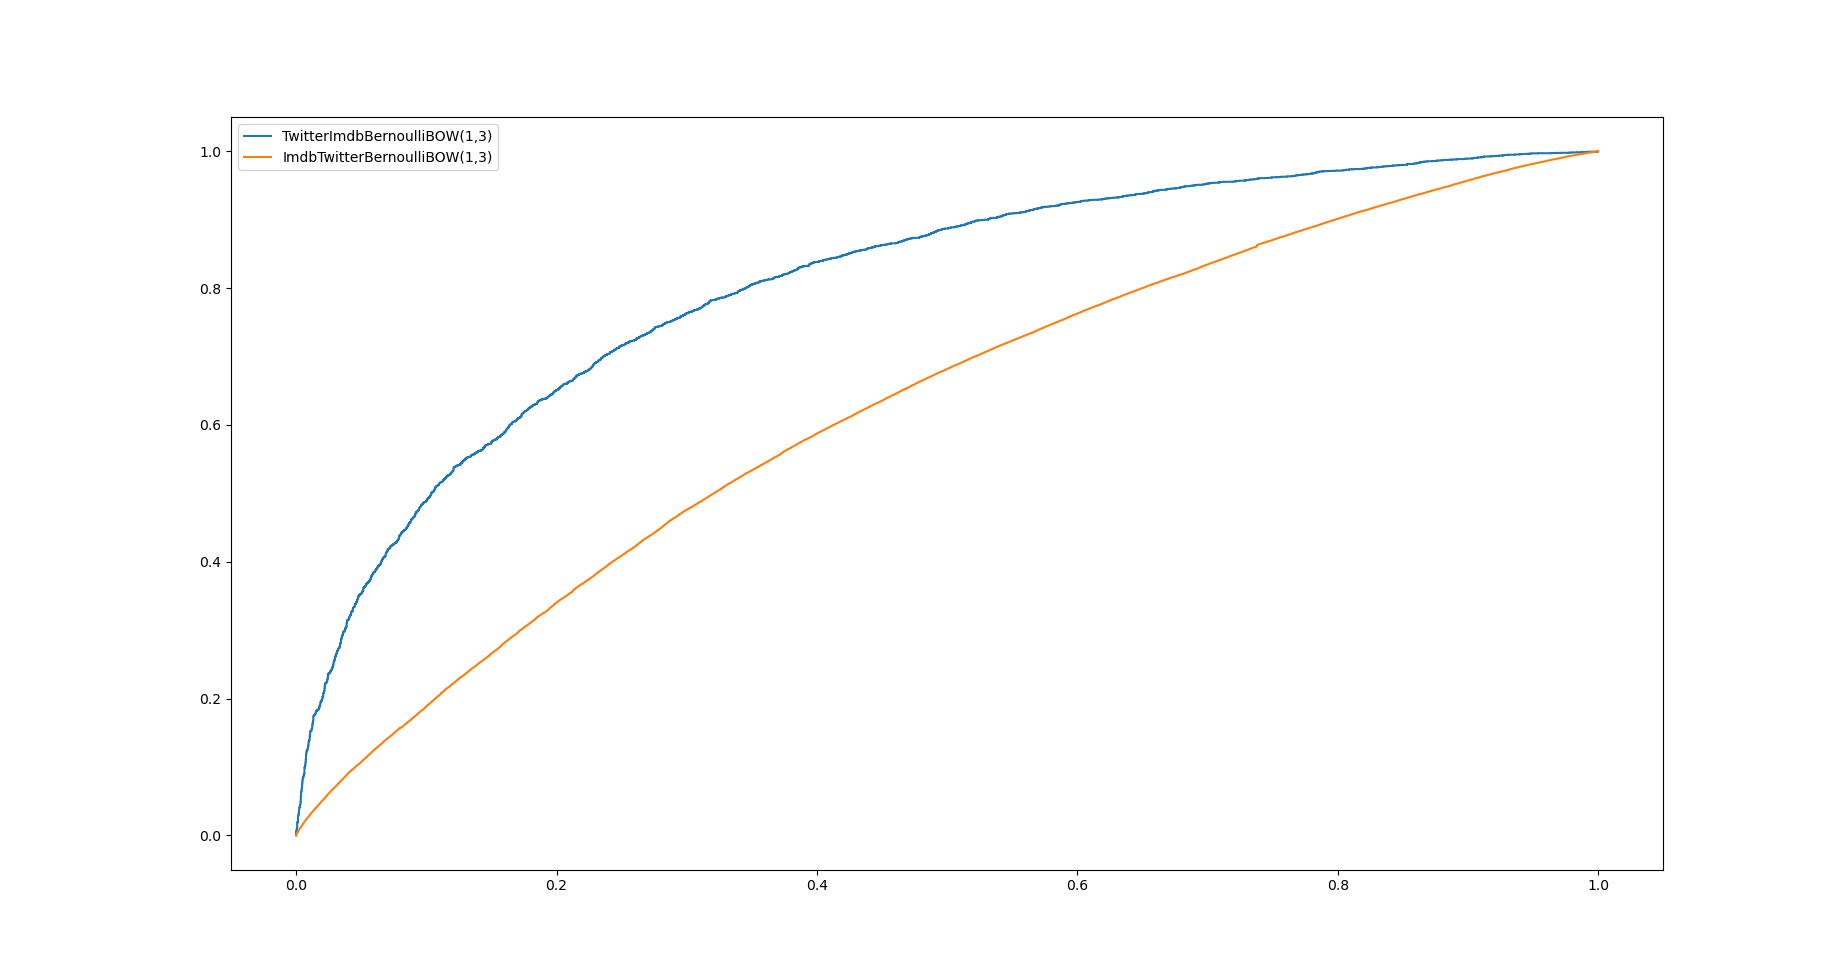
\includegraphics[scale=0.3]{../experiments/plots/ImdbTwitter}
        \caption{Comparison between Imdb-Twitter (training on Imdb, testing on Twitter) and Twitter-Imdb (training on Twitter, testing on Imdb).}
        \label{fig:TwitterImdb}        
    \end{figure}
    
    \begin{figure}[h!t]
        \centering
        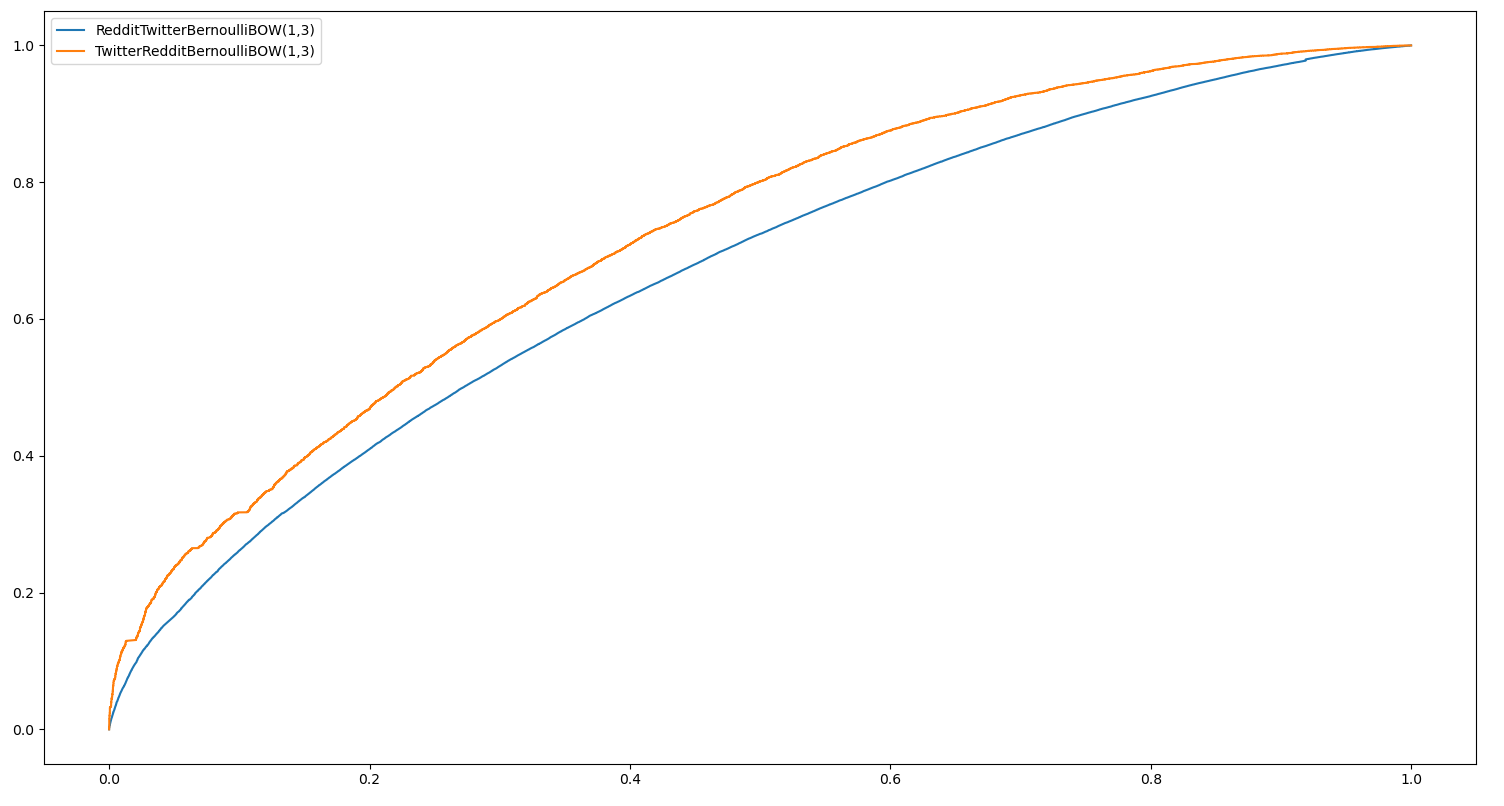
\includegraphics[scale=0.3]{../experiments/plots/RedditTwitter}
        \caption{Comparison betwen Reddit-Twitter (training on Reddit, testing on Twitter), and Twitter-Reddit (training on Twitter, testing on Reddit).}
        \label{fig:TwitterReddit}
    \end{figure}
    
    This is something usually not done since different datasets will have different distributions hence we expect bad results and this is what we got except for one particular case.
    Training our model with the Twitter dataset and testing it with the IMDb one strangely gives us rather good metrics, this can be seen in table \ref{tab:versus_metrics} where only the comparision betwen Twitter and IMDb is shown since results are more interesting. 
    
    This could be due to Twitter's dataset being very large while other datasets are smaller and also very specific.
    The Reddit one is only about a specific set of american football games and the IMDb one is about cinematographic reviews, reasonably in this case lexicon is also more specific than arbitrairly picked tweets.
    On the other hand Sentiment140 covers a wider class of human language and is less prone to be biased.
    
    
    \begin{table}[h!t]
        \centering
        \caption{Comparing metrics for some train test combinations (using Bernoulli event model). Twitter-IMDb is surprisingly not bad (even though still lower than training and testing directly on IMDb)}
        \label{tab:versus_metrics}
        \begin{tabular}{c|ccc}
            \hline
            Train-Test & Accuracy & F1 & AUROC \\
            \hline 
            Twitter-IMDb & 0.732 & 0.723 & 0.806 \\ 
            IMDb-IMDb & 0.891 & 0.887 & 0.963 \\ 
            IMDb-Twitter & 0.550 & 0.330 & 0.625 \\ 
            Twitter-Twitter & 0.797 & 0.799 & 0.880 \\ 
            \hline
        \end{tabular}
    \end{table}
    
    \section*{Conclusions}
    One of the main conclusions that can be drawn from our experiments is that preprocessing must be done really carefully, we noticed that performing no preprocessing at all was better than performing spaCy's lemmatization and stopwords removal. 
    It is interesting to note that also some of the most performing Kaggle's notebook improved their performance after removing some preprocessing from their pipeline (in particular the stopwords removal), this testifies how difficult is to get the preprocessing right.
    
    The model giving us the best results is the multinomial na\"ive Bayes with tf-idf (without preprocessing or with just some ad-hoc stopwords removal), we were in general surprised of how using FastText performs worse than the classical approaches; the reason we gave to this phenomenon is that  more complex models than na\"ive Bayes, such as neural networks, are required in order to get the best out of word embeddings; also na\"ive Bayes works better with more classical and simple representations. 
    Comparing our model to some models from Kaggle, we observed that, at least in this context, na\"ive Bayes can give competitive results even compared to models like LSTM, which is really surprising considered its simplicity.

    \section*{Work distribution}
    Broadly these are the principal fields in which each member contributed:

    \begin{itemize}
        \item \textbf{Tommaso Battistini}: Embeddings, gaussian na\"ive Bayes.
        \item \textbf{Edoardo De Matteis}: Classical na\"ive Bayes, tests.
        \item \textbf{Leonardo Emili}: Preprocessing, stopword investigation.
        \item \textbf{Mirko Giacchini}: Na\"ive Bayes models, tests.
        \item \textbf{Alessio Luciani}: Na\"ive Bayes models, tests.
    \end{itemize}

    Each member reviewed other one's code and contributed resolving bugs, reviewing resources and sharing ideas. 

    \bibliography{main}{}
    \bibliographystyle{plainurl}

\end{document}